\documentclass{article}

\usepackage[margin=2cm]{geometry}
\usepackage{graphicx}
\usepackage{graphics}
\usepackage{hyperref}
\usepackage{psfrag}
\usepackage{ifthen}
\usepackage{array}
\usepackage{longtable}
\usepackage{color}
\usepackage{tikz}
\usepackage{amsmath, amsfonts, amsthm}
\usepackage[shortlabels]{enumitem}
\setcounter{secnumdepth}{0}
\newcommand{\N}{\mathbb{N}}
\newcommand{\R}{\mathbb{R}}

\usetikzlibrary{svg.path}


\begin{document}

\title{Homework 3}
\author{Hayden Pott}
\date{15 April 2024}

\maketitle

\section{2-2}
Consider the following model.
\begin{itemize}
    \item The objects under consideration are the points in the plane.
    \item The sets under consideration are the straight lines in the plane.
    \item An object (point) belongs to a set (line) iff the point is on the line.
\end{itemize}

\begin{enumerate}[a)]
    \item Explain why the model satisfies Axioms 2.1 and 2.2. \\
        \textbf{ANSWER:} The model satisfies axiom 2.1 by stating that there are
        sets, in this case the straight lines in the plane.  The model also
        satisfies axiom 2.2 by the third thing it states, allowing us to see
        whether an object/point is in the set/line by checking whether that
        point is on the line.
    \item Can it be determined if two sets have elements in common? \\
        \textbf{ANSWER:} Yes, we can determine if two sets have elements in
        common by checking if that element is in \textit{both} sets.
    \item If two sets have elements in common, must the collection of common
        elements be a set? \\
        \textbf{ANSWER:} Yes, the collection of common elements must be a set
        since we have the ability to check whether an object appears in this
        collection, satisfying Axiom 2.1.  We can satisfy Axiom 2.1 by stating
        that it is a set.
\end{enumerate}

\section{2-3}
For each of the following situations, sketch a Venn diagram
\begin{enumerate}[a)]
    \item Three sets so that any two of them overlap and so that all three
        overlap.  None of the overlaps of two sets is completely contained in
        another overlap of two or more sets. \\
        \textbf{ANSWER:} \\
        \begin{center}
            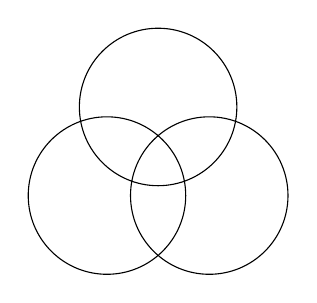
\begin{tikzpicture}
                \draw (90:.75) circle (1)
                    (210:.75) circle (1)
                    (330:.75) circle (1);
            \end{tikzpicture}
        \end{center}

        \newpage

    \item Four sets so that any two of them overlap, any three of them overlap
        and so that all four overlap.  None of the overlaps of two sets is
        completely contained in another overlap of two or more sets.  None of
        the overlaps of three sets is completely contained in another overlap of
        three or more sets. \\
        \textbf{ANSWER:} \\
        \begin{center}
            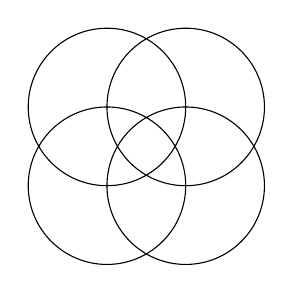
\begin{tikzpicture}
                \draw (0,0) circle (1)
                    (0,1) circle (1)
                    (1,0) circle (1)
                    (1,1) circle (1);
            \end{tikzpicture}
        \end{center}
\end{enumerate}

\section{2-6}
Let $A$, $B$, and $U$ be sets so that $A\subseteq U$ and $B \subseteq U$.  Prove
that $A \subseteq B$ iff $(U \setminus B) \subseteq (U \setminus A)$. \\
\textbf{ANSWER:}
\begin{proof} \hfill
\item[$\implies$] Let $A \subseteq B$.  Let $x \in U \setminus B$ be ABF.
    \begin{align*}
        &\implies x \not\in B \\
        &\implies x \not\in A \\
        &\implies x \in U \setminus A \\
        &\implies (U \setminus B) \subseteq (U \setminus A)
    \end{align*}
\item[$\impliedby$] Let $(U \setminus B) \subseteq (U \setminus A$.  Let
    $x \in A$ be ABF.
    \begin{align*}
        &\implies x \not\in (U \setminus A) \\
        &\implies x \not\in (U \setminus B) \\
        &\implies x \in B \\
        &\implies A \subseteq B \\
    \end{align*}
    Therefore, $A \subseteq B \iff (U \setminus B) \subseteq (U \setminus A)$
\end{proof}

\section{2-10}
Let $A$, $B$ be sets.  Prove that $A \setminus (A \setminus B) = A \cap B$. \\
\textbf{ANSWER:}
\begin{proof} \hfill \newline
    Let $\mathcal{C} := \{A, B\}$.
    \begin{align*}
        A \setminus (A \setminus B)
        &= \{x \in A : x \not\in (A \setminus B)\} \\
        &= \{x \in A : x \not\in \{y \in A : y \not\in B\}\} \\
        &= \{x \in A : \neg(x \not\in B)\} \\
        &= \{x \in A : x \in B\} \\
        &= \{x \in A : x \in A \land x \in B\} \\
        &= \{x \in A : [\forall C \in \mathcal{C} : x \in C]\} \\
        &= \bigcap \mathcal{C} \\
        &= A \cap B
    \end{align*}
\end{proof}

\section{2-11}
Let $A$, $B$ be sets.  Sketch a Venn diagram that illustrates the equation $A
\setminus (A \setminus B) = A \cap B$ \\
\textbf{ANSWER:} \\
\begin{center}
    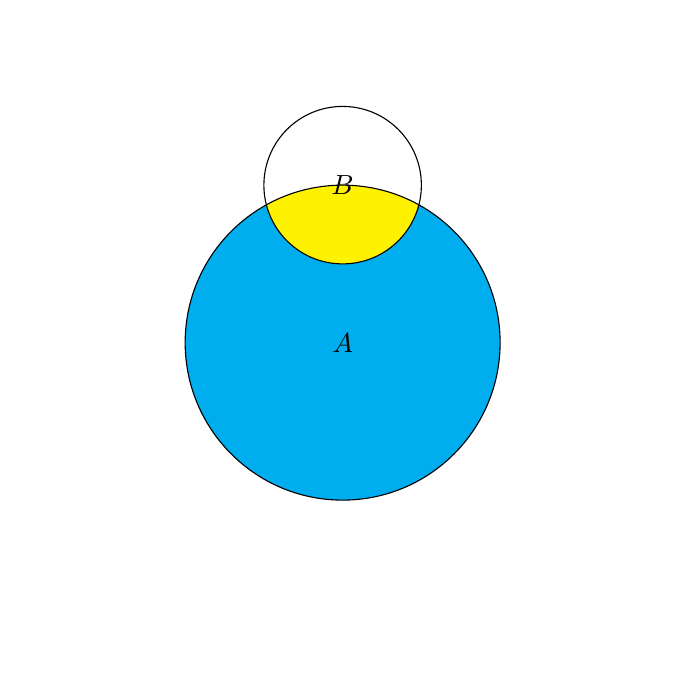
\begin{tikzpicture}
        \def\A{(0,0) circle (2)}
        \def\B{(0,2) circle (1)}

        \begin{scope}
            \clip (-4,-4) rectangle (4,4) \B;
            \fill[cyan] \A;
        \end{scope}
        \begin{scope}
            \clip \A;
            \fill[yellow] \B;
        \end{scope}
        \draw \A node[text=black] {$A$};
        \draw \B node [text=black] {$B$};
    \end{tikzpicture} \\
    Cyan: $A \setminus B$ \\
    Yellow $A \setminus (A \setminus B)$ or $A \cap B$ \\
\end{center}

\end{document}
